\documentclass[11pt]{article}

\usepackage[utf8]{inputenc}
\usepackage[T1]{fontenc}
\usepackage[spanish]{babel}
\usepackage{amsmath}
\usepackage{amssymb}
\usepackage{booktabs}
\usepackage{array}
\usepackage{longtable}
\usepackage{graphicx}
\usepackage{float}
\usepackage{geometry}

\geometry{letterpaper, margin=2.5cm}

\title{Resultados, Discusi\'on y Conclusiones Finales}
\author{Proyecto Capstone FinPUC}
\date{Junio 2026}

\begin{document}

\maketitle

\section{An\'alisis de Resultados fuera de Muestra}

\subsection{Evaluaci\'on en ventanas m\'oviles y test limpio}

La evaluaci\'on final se realiz\'o bajo la arquitectura de tres horizontes temporales definida para prevenir \textit{overfitting}. En particular, los resultados reportados en esta secci\'on corresponden al Horizonte 3, utilizado como test limpio y no observado durante la calibraci\'on de los par\'ametros de Black--Litterman. Esta separaci\'on permite interpretar los KPIs financieros como evidencia fuera de muestra estricta, ya que la configuraci\'on final del modelo fue congelada antes de ejecutar la evaluaci\'on econ\'omica.

La comparaci\'on se realiza entre tres referencias: Markowitz base, Black--Litterman calibrado y benchmark equiponderado. Markowitz representa el caso base param\'etrico; Black--Litterman incorpora la \textit{view} macro calibrada; y el benchmark equiponderado funciona como control no optimizado, independiente de estimaciones de retornos esperados.

\begin{table}[H]
\centering
\caption{Comparaci\'on fuera de muestra en Horizonte 3}
\label{tab:kpis_test}
\begin{tabular}{l l r r r r}
\toprule
Escenario & Modelo / Perfil & Ventanas & Sharpe & Drawdown & Comentario \\
\midrule
Con pandemia & BL, Arriesgado & 4 & 1.644 & -11.1\% & Mejora Sharpe 19.9\% \\
Con pandemia & Markowitz, Arriesgado & 4 & 1.391 & -18.7\% & Caso base \\
Con pandemia & Benchmark & 4 & 1.309 & -16.8\% & Control equiponderado \\
\midrule
Con pandemia & BL, Muy arriesgado & 4 & 1.119 & -22.8\% & Mejora Sharpe 23.1\% \\
Con pandemia & Markowitz, Muy arriesgado & 4 & 0.933 & -27.6\% & Caso base \\
\midrule
Sin pandemia & BL, Arriesgado & 1 & 1.562 & -12.1\% & Mejora Sharpe 3.2\% \\
Sin pandemia & Markowitz, Arriesgado & 1 & 1.513 & -18.2\% & Caso base \\
Sin pandemia & Benchmark & 1 & 1.290 & -16.8\% & Control equiponderado \\
\bottomrule
\end{tabular}
\end{table}

La Tabla \ref{tab:kpis_test} muestra que el aporte principal de Black--Litterman calibrado aparece en los perfiles de mayor exposici\'on al riesgo, especialmente en el escenario con pandemia. En el perfil Arriesgado, el modelo calibrado mejora simult\'aneamente el Sharpe y el drawdown frente a Markowitz. En el perfil Muy arriesgado ocurre el mismo patr\'on: la mejora porcentual de Sharpe se combina con una reducci\'on de la profundidad de las p\'erdidas. Esta evidencia es consistente con la tesis metodol\'ogica del proyecto: Black--Litterman no se incorpora para maximizar retorno bruto en todos los casos, sino para estabilizar la recomendaci\'on cuando Markowitz queda m\'as expuesto al error de estimaci\'on.

La Figura \ref{fig:sharpe_rolling} ilustra la evoluci\'on temporal del Sharpe en las ventanas de test limpio para el perfil Arriesgado en el escenario con pandemia. La visualizaci\'on permite observar que la mejora no proviene de una sola medici\'on aislada, sino de un comportamiento comparativo m\'as estable a trav\'es de las ventanas fuera de muestra.

\begin{figure}[H]
\centering
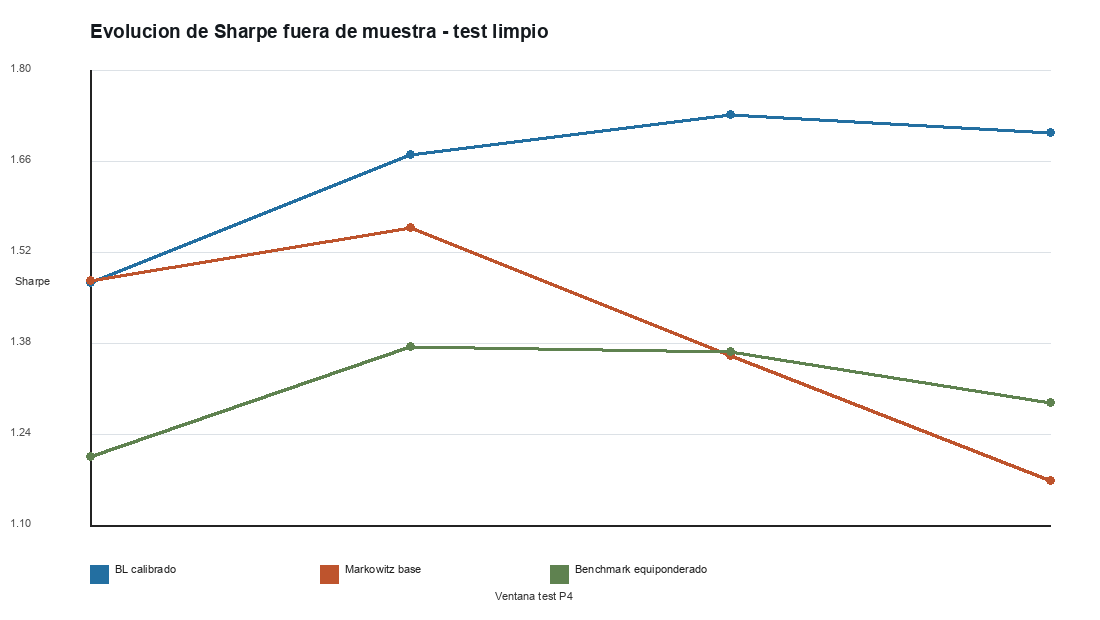
\includegraphics[width=0.8\textwidth]{figuras/grafico_sharpe.png}
\caption{Evoluci\'on temporal del Sharpe fuera de muestra en el Horizonte 3. La figura compara Black--Litterman calibrado, Markowitz base y benchmark equiponderado bajo ventanas m\'oviles.}
\label{fig:sharpe_rolling}
\end{figure}

\subsection{Lectura detallada por perfil de riesgo}

La recomendaci\'on no es homog\'enea para todos los perfiles. Para evitar una conclusi\'on agregada que esconda diferencias relevantes, se separa el an\'alisis por escenario y por perfil de riesgo. Esta lectura es especialmente importante porque la calibraci\'on de Black--Litterman modifica la exposici\'on al riesgo de forma distinta seg\'un la aversi\'on al riesgo del cliente. En perfiles conservadores, la restricci\'on de volatilidad y de peso m\'aximo ya limita la agresividad de Markowitz; por ello, el margen de mejora de Black--Litterman es menor. En perfiles agresivos, en cambio, Markowitz queda m\'as expuesto a errores de estimaci\'on, por lo que el prior de equilibrio y la \textit{view} macro pueden aportar mayor estabilizaci\'on.

\begin{table}[H]
\centering
\caption{Desempe\~no por perfil en escenario con pandemia}
\label{tab:perfiles_con_pandemia}
\begin{tabular}{l r r r r r}
\toprule
Perfil & Sharpe BL & Sharpe MK & Mejora Sharpe & DD BL & DD MK \\
\midrule
Muy conservador & 1.625 & 1.699 & -4.4\% & -9.1\% & -9.0\% \\
Conservador & 1.638 & 1.749 & -6.5\% & -9.2\% & -9.0\% \\
Neutro & 1.660 & 1.773 & -6.0\% & -9.4\% & -10.9\% \\
Arriesgado & 1.644 & 1.391 & 19.9\% & -11.1\% & -18.7\% \\
Muy arriesgado & 1.119 & 0.933 & 23.1\% & -22.8\% & -27.6\% \\
\bottomrule
\end{tabular}
\end{table}

En el escenario con pandemia, la Tabla \ref{tab:perfiles_con_pandemia} muestra una separaci\'on clara entre perfiles conservadores e intensivos en riesgo. En Muy conservador y Conservador, Black--Litterman no mejora el Sharpe promedio respecto de Markowitz y tampoco entrega una mejora material de drawdown. Esto indica que, cuando la cartera ya est\'a fuertemente limitada por restricciones de riesgo, el beneficio marginal de incorporar la \textit{view} macro es acotado. En el perfil Neutro aparece una lectura mixta: Markowitz conserva mayor Sharpe, pero Black--Litterman reduce el drawdown promedio. Esto sugiere que BL puede funcionar como alternativa defensiva, aunque no como recomendaci\'on dominante.

El resultado cambia en Arriesgado y Muy arriesgado. En ambos casos, Black--Litterman mejora el Sharpe y reduce el drawdown frente a Markowitz. La mejora no se explica solo por mayor retorno ajustado por volatilidad, sino por una reducci\'on relevante de la ca\'ida m\'axima. Esta es la evidencia m\'as fuerte a favor de recomendar Black--Litterman en perfiles con mayor exposici\'on al riesgo durante escenarios de estr\'es.

\begin{table}[H]
\centering
\caption{Desempe\~no por perfil en escenario sin pandemia}
\label{tab:perfiles_sin_pandemia}
\begin{tabular}{l r r r r r}
\toprule
Perfil & Sharpe BL & Sharpe MK & Mejora Sharpe & DD BL & DD MK \\
\midrule
Muy conservador & 1.738 & 1.736 & 0.2\% & -10.2\% & -10.3\% \\
Conservador & 1.718 & 1.728 & -0.6\% & -10.1\% & -11.0\% \\
Neutro & 1.664 & 1.747 & -4.8\% & -10.2\% & -13.0\% \\
Arriesgado & 1.562 & 1.513 & 3.2\% & -12.1\% & -18.2\% \\
Muy arriesgado & 1.154 & 1.198 & -3.7\% & -21.1\% & -26.5\% \\
\bottomrule
\end{tabular}
\end{table}

En el escenario sin pandemia, la Tabla \ref{tab:perfiles_sin_pandemia} muestra una mejora m\'as moderada. El perfil Arriesgado vuelve a favorecer a Black--Litterman, aunque con una magnitud menor que en pandemia. En Neutro y Muy arriesgado, Markowitz conserva mayor Sharpe, pero Black--Litterman reduce el drawdown. Esta combinaci\'on confirma que el modelo calibrado tiene un sesgo defensivo: no siempre maximiza Sharpe, pero tiende a contener p\'erdidas. Por ello, la recomendaci\'on debe distinguir entre clientes que priorizan retorno ajustado por volatilidad y clientes que priorizan protecci\'on frente a ca\'idas.

\begin{figure}[H]
\centering
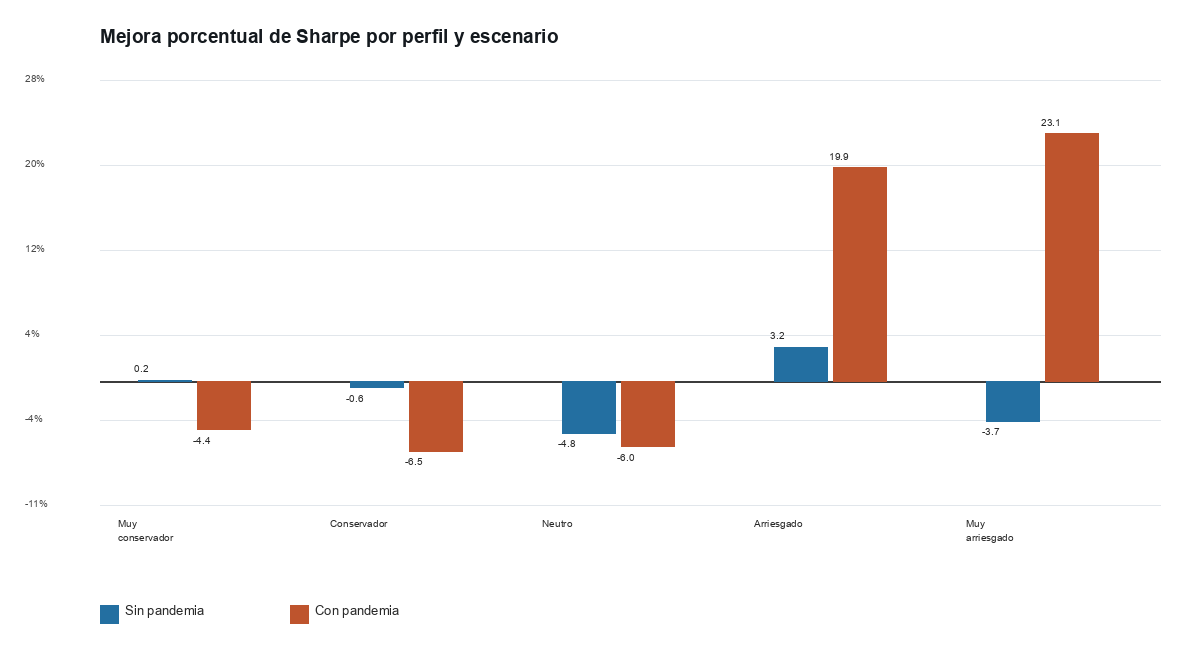
\includegraphics[width=0.8\textwidth]{figuras/mejora_sharpe_perfiles.png}
\caption{Mejora porcentual del Sharpe de Black--Litterman frente a Markowitz por perfil de riesgo y escenario.}
\label{fig:mejora_sharpe_perfiles}
\end{figure}

La Figura \ref{fig:mejora_sharpe_perfiles} resume visualmente la principal conclusi\'on del an\'alisis por perfil: la mejora de Sharpe se concentra en los perfiles Arriesgado y Muy arriesgado, especialmente en el escenario con pandemia. En los perfiles de menor riesgo, la ganancia de BL no es sistem\'atica, lo que refuerza la necesidad de una recomendaci\'on segmentada.

\begin{figure}[H]
\centering
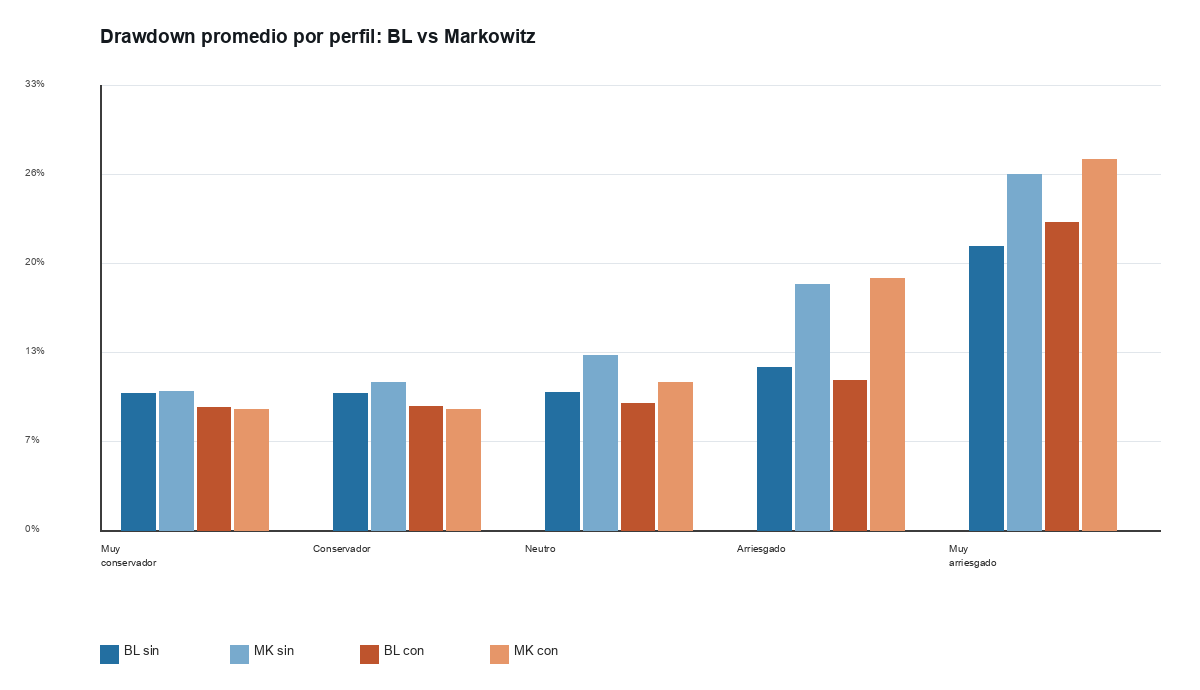
\includegraphics[width=0.8\textwidth]{figuras/drawdown_perfiles.png}
\caption{Comparaci\'on de drawdown promedio por perfil, modelo y escenario. Barras menores representan menor profundidad de p\'erdidas.}
\label{fig:drawdown_perfiles}
\end{figure}

La Figura \ref{fig:drawdown_perfiles} complementa el an\'alisis de Sharpe. Incluso cuando BL no domina en Sharpe, en varios perfiles reduce la magnitud del drawdown. Esto es especialmente visible en Arriesgado y Muy arriesgado. Por tanto, la discusi\'on no debe centrarse exclusivamente en Sharpe, sino en el balance entre desempe\~no ajustado por riesgo y resiliencia ante p\'erdidas.

\begin{table}[H]
\centering
\caption{Recomendaci\'on emp\'irica por perfil de riesgo}
\label{tab:recomendacion_perfil}
\begin{tabular}{p{0.20\linewidth} p{0.28\linewidth} p{0.42\linewidth}}
\toprule
Perfil & Modelo recomendado & Fundamento emp\'irico \\
\midrule
Muy conservador & Markowitz / BL defensivo & Diferencias marginales; Markowitz mantiene simplicidad y buen Sharpe. \\
Conservador & Markowitz & BL no mejora Sharpe de forma consistente y P4 favorece el saldo de Markowitz. \\
Neutro & Markowitz, con BL como alternativa defensiva & Markowitz domina Sharpe y P4; BL puede reducir drawdown. \\
Arriesgado & Black--Litterman calibrado & Mejora Sharpe en ambos escenarios y reduce drawdown de forma marcada. \\
Muy arriesgado & Black--Litterman en estr\'es; Markowitz en normalidad & BL mejora en pandemia; Markowitz conserva Sharpe en sin pandemia. \\
\bottomrule
\end{tabular}
\end{table}

La Tabla \ref{tab:recomendacion_perfil} resume la recomendaci\'on segmentada. El criterio no es escoger un modelo universal, sino identificar cu\'ando la estructura bayesiana de Black--Litterman agrega valor frente al caso base. Esta distinci\'on responde directamente al feedback metodol\'ogico: el informe final no debe forzar una conclusi\'on de dominancia global, sino justificar qu\'e modelo es preferible seg\'un perfil, escenario y objetivo.

\section{Resultados de la Din\'amica del Portafolio}

\subsection{Turnover semestral e implementabilidad}

Adem\'as de evaluar KPIs financieros agregados, se analizaron m\'etricas de din\'amica del portafolio. El turnover semestral permite medir cu\'anto debe transarse en cada rebalanceo para pasar desde el portafolio con deriva natural de mercado hacia el nuevo portafolio objetivo. Esta m\'etrica es relevante porque una estrategia con buen Sharpe pero excesiva rotaci\'on puede ser poco implementable para un recomendador real.

\begin{table}[H]
\centering
\caption{Turnover y concentraci\'on de Black--Litterman por perfil en test limpio}
\label{tab:turnover}
\begin{tabular}{l l r r r}
\toprule
Escenario & Perfil & Turnover medio & N efectivo & HHI sectorial \\
\midrule
Con pandemia & Muy conservador & 6.3\% & 112.6 & 0.169 \\
Con pandemia & Conservador & 6.2\% & 118.1 & 0.166 \\
Con pandemia & Neutro & 6.4\% & 136.3 & 0.158 \\
Con pandemia & Arriesgado & 7.0\% & 205.7 & 0.135 \\
Con pandemia & Muy arriesgado & 9.9\% & 121.0 & 0.214 \\
\midrule
Sin pandemia & Muy conservador & 7.0\% & 221.2 & 0.147 \\
Sin pandemia & Conservador & 7.0\% & 233.5 & 0.144 \\
Sin pandemia & Neutro & 6.9\% & 271.1 & 0.137 \\
Sin pandemia & Arriesgado & 6.9\% & 360.5 & 0.124 \\
Sin pandemia & Muy arriesgado & 9.2\% & 163.3 & 0.178 \\
\bottomrule
\end{tabular}
\end{table}

La Tabla \ref{tab:turnover} indica que el turnover promedio de Black--Litterman se mantiene en rangos operativamente moderados para todos los perfiles. Esto es importante para FinPUC porque la recomendaci\'on no solo debe ser estad\'isticamente defendible, sino tambi\'en ejecutable por un cliente real. El perfil Muy arriesgado presenta la mayor rotaci\'on y la mayor concentraci\'on sectorial relativa en ambos escenarios, lo que es coherente con una cartera que acepta mayor exposici\'on activa. En cambio, los perfiles conservadores muestran rotaci\'on baja, aunque con menor n\'umero efectivo de activos que el perfil Arriesgado, reflejando una cartera m\'as restringida por l\'imites de riesgo.

\subsection{Drift de pesos y estabilidad de composici\'on}

La estabilidad de composici\'on fue evaluada comparando la estructura sectorial inicial y final de las carteras dentro de las ventanas de test. La Figura \ref{fig:drift_pesos} muestra el drift sectorial de pesos para Black--Litterman en una ventana representativa del escenario con pandemia. Este an\'alisis permite identificar si el modelo mantiene una exposici\'on relativamente persistente o si depende de cambios bruscos entre rebalanceos.

\begin{figure}[H]
\centering
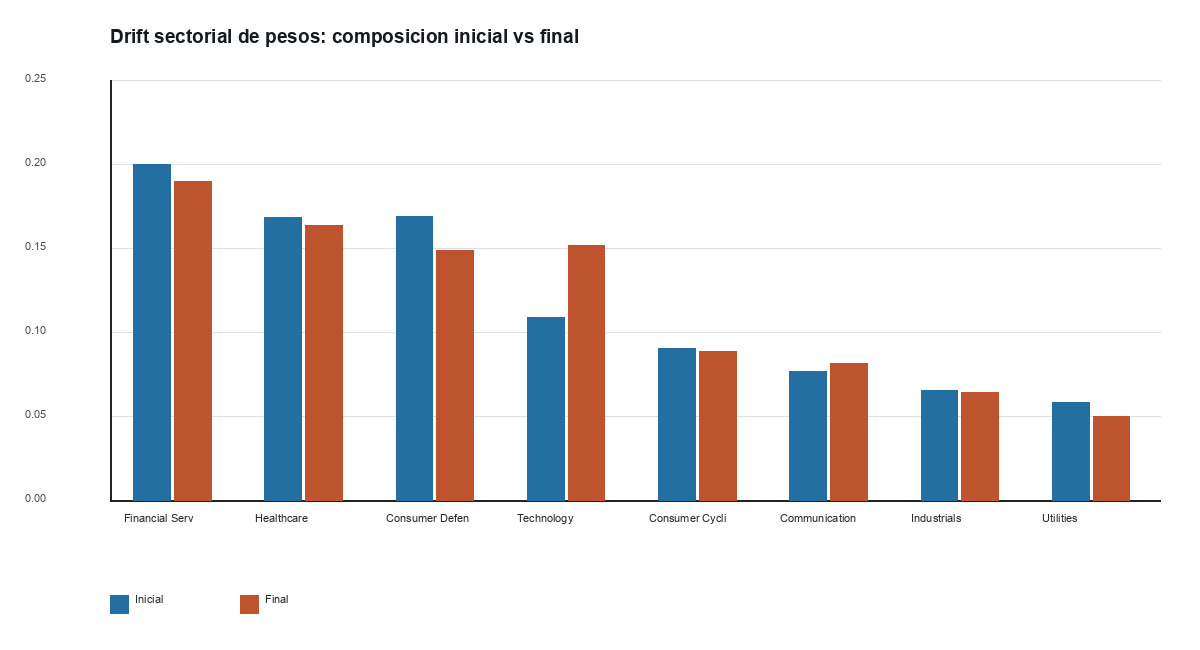
\includegraphics[width=0.8\textwidth]{figuras/drift_pesos.png}
\caption{Comparaci\'on de composici\'on sectorial inicial y final del portafolio Black--Litterman calibrado. La figura permite visualizar el drift de pesos generado por rebalanceos sucesivos.}
\label{fig:drift_pesos}
\end{figure}

El resultado sugiere que la cartera no se comporta como una estrategia puramente especulativa de alta rotaci\'on. Aunque existen ajustes sectoriales entre el inicio y el final de la ventana, el patr\'on general mantiene una diversificaci\'on econ\'omica amplia. Esta lectura complementa el turnover: una baja rotaci\'on promedio y una composici\'on razonablemente estable fortalecen la implementabilidad del modelo.

\subsection{Concentraci\'on sectorial de retornos}

El an\'alisis de concentraci\'on sectorial distingue entre diversificaci\'on por n\'umero de activos y diversificaci\'on por fuente de retorno. Un portafolio puede contener muchos activos, pero si la mayor parte del retorno proviene de uno o dos sectores, su riesgo econ\'omico efectivo sigue siendo concentrado. Para medirlo, se calcul\'o la participaci\'on absoluta de los principales sectores en la contribuci\'on total de retornos.

\begin{figure}[H]
\centering
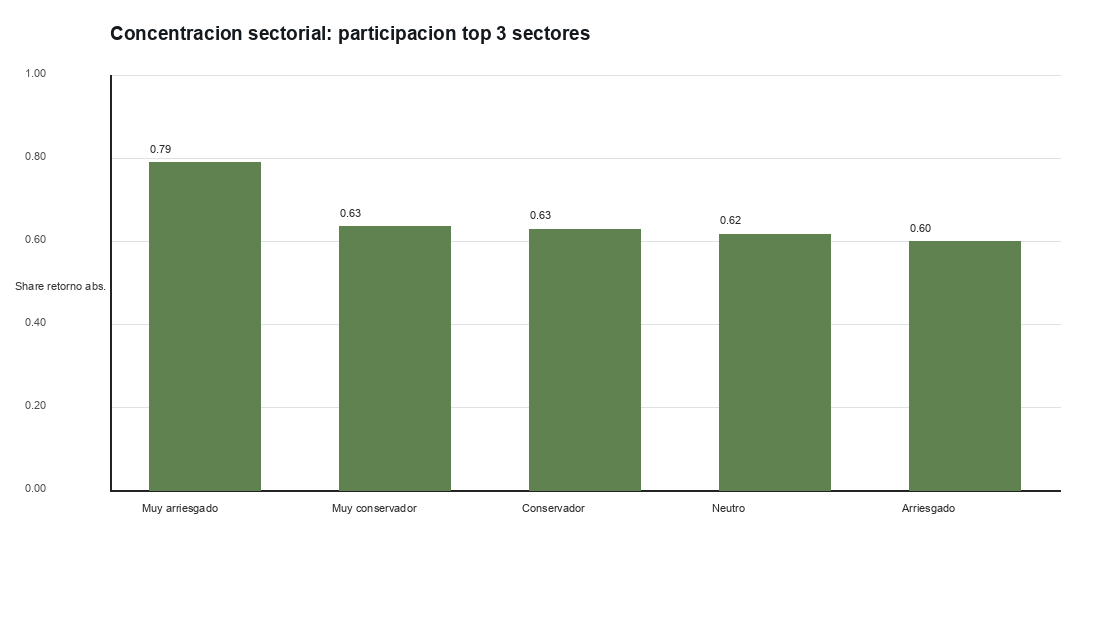
\includegraphics[width=0.8\textwidth]{figuras/distribucion_sectorial.png}
\caption{Concentraci\'on sectorial de retornos medida como participaci\'on absoluta acumulada de los tres sectores principales.}
\label{fig:sectorial}
\end{figure}

La Figura \ref{fig:sectorial} muestra que la concentraci\'on sectorial aumenta en los perfiles m\'as riesgosos. Este resultado no invalida la recomendaci\'on, pero s\'i entrega una advertencia relevante para la presentaci\'on final: Black--Litterman reduce drawdowns en perfiles agresivos, pero parte de ese resultado puede depender de exposiciones sectoriales espec\'ificas. Por ello, la recomendaci\'on debe acompa\~narse de monitoreo de concentraci\'on.

\section{Evaluaci\'on Econ\'omica Monte Carlo P4 en Horizonte Limpio}

\subsection{Resultados cliente--empresa}

La evaluaci\'on P4 se ejecut\'o exclusivamente en el Horizonte 3. Esto implica que las variables de riqueza terminal, tasa de retiro, probabilidad de ganancia y utilidad de empresa se calculan despu\'es de la optimizaci\'on del portafolio. La utilidad corporativa no forma parte de la funci\'on objetivo de Markowitz ni de Black--Litterman; es una consecuencia ex-post del saldo administrado y del comportamiento simulado del cliente.

\begin{table}[H]
\centering
\caption{Score P4 por perfil y escenario en test limpio}
\label{tab:p4}
\begin{tabular}{l l r r r r}
\toprule
Escenario & Perfil & Riqueza BL & Score BL & Riqueza MK & Score MK \\
\midrule
Con pandemia & Muy conservador & 1534 & 973 & 1593 & 1060 \\
Con pandemia & Conservador & 2241 & 2278 & 2369 & 2427 \\
Con pandemia & Neutro & 2124 & 2243 & 2623 & 2792 \\
Con pandemia & Arriesgado & 1248 & 1255 & 2067 & 2119 \\
Con pandemia & Muy arriesgado & 1096 & 1097 & 1535 & 1540 \\
\midrule
Sin pandemia & Muy conservador & 1695 & 1159 & 1725 & 1212 \\
Sin pandemia & Conservador & 2452 & 2475 & 2508 & 2546 \\
Sin pandemia & Neutro & 2291 & 2428 & 2797 & 2982 \\
Sin pandemia & Arriesgado & 1241 & 1247 & 2173 & 2230 \\
Sin pandemia & Muy arriesgado & 1067 & 1068 & 1739 & 1748 \\
\bottomrule
\end{tabular}
\end{table}

La Tabla \ref{tab:p4} muestra que Markowitz mantiene una ventaja sistem\'atica en riqueza terminal y score P4. Esta diferencia no invalida la mejora financiera observada en Sharpe y drawdown para perfiles agresivos; m\'as bien revela la tensi\'on econ\'omica central del proyecto. Black--Litterman calibrado reduce ca\'idas en los perfiles de mayor riesgo, pero esa postura m\'as defensiva puede traducirse en menor crecimiento esperado, menor saldo administrado y, por lo tanto, menor utilidad ex-post para la empresa. La recomendaci\'on final debe explicitar esta diferencia: BL mejora resiliencia de portafolio en segmentos espec\'ificos, mientras que Markowitz puede ser superior cuando el objetivo dominante es maximizar riqueza terminal o score comercial.

\begin{figure}[H]
\centering
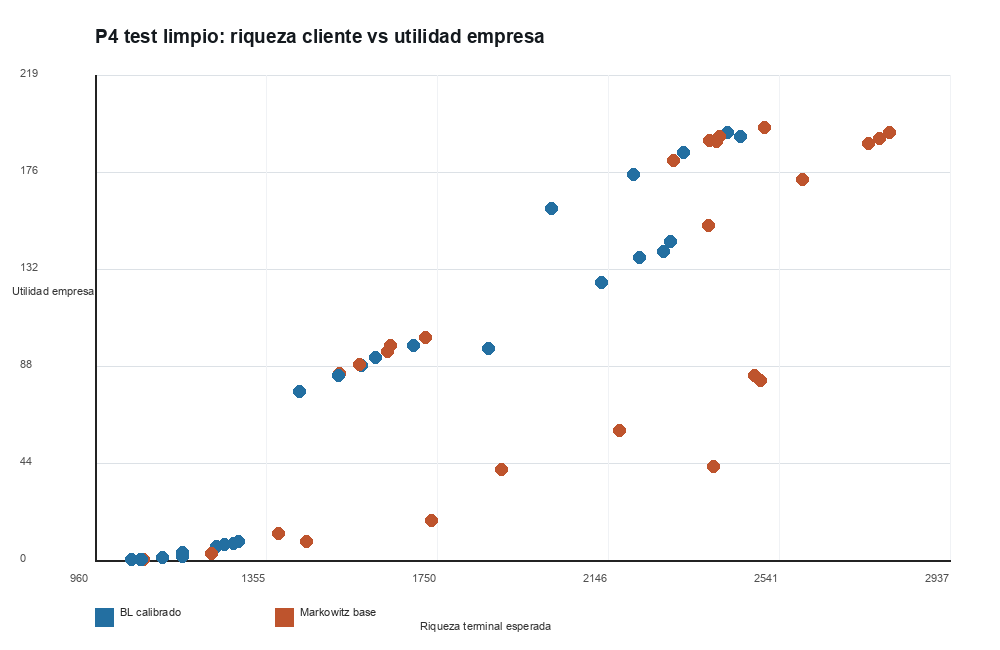
\includegraphics[width=0.8\textwidth]{figuras/distribucion_p4.png}
\caption{Relaci\'on entre riqueza terminal esperada del cliente y utilidad ex-post de la empresa en la simulaci\'on Monte Carlo P4.}
\label{fig:p4_scatter}
\end{figure}

La Figura \ref{fig:p4_scatter} evidencia la relaci\'on positiva entre riqueza terminal y utilidad de la empresa por saldo administrado. Esta relaci\'on refuerza la necesidad de separar objetivos: el portafolio debe optimizarse para el cliente, mientras que la utilidad de FinPUC debe evaluarse posteriormente como impacto de negocio. Incorporar la utilidad corporativa directamente en el optimizador habr\'ia contaminado el objetivo financiero del cliente.

\section{Discusi\'on de Robustez}

\subsection{Cumplimiento del feedback metodol\'ogico}

La nueva arquitectura responde directamente a las observaciones del profesor del 9 de junio. Primero, la separaci\'on en tres horizontes elimina la objeci\'on de usar la misma ventana para calibrar y testear P4. Segundo, las ventanas m\'oviles aumentan el n\'umero de observaciones fuera de muestra y permiten observar distintos reg\'imenes temporales. Tercero, las m\'etricas de estabilidad del portafolio incorporan una dimensi\'on operacional que no estaba capturada por Sharpe, retorno o drawdown.

La principal consecuencia interpretativa es que la conclusi\'on se vuelve m\'as matizada, pero tambi\'en m\'as defendible. Black--Litterman calibrado no domina universalmente a Markowitz ni al benchmark. Su valor aparece en segmentos espec\'ificos: perfiles con mayor tolerancia al riesgo y escenarios donde el error de estimaci\'on de Markowitz se traduce en ca\'idas m\'as profundas.

\subsection{Robustez como resiliencia, no dominancia universal}

La evidencia debe leerse bajo el concepto de resiliencia. Un modelo robusto no es necesariamente aquel que obtiene el mayor Sharpe en todas las ventanas, sino aquel que mantiene desempe\~no razonable y controla p\'erdidas en condiciones adversas. En este sentido, Black--Litterman aporta una estructura bayesiana que suaviza la dependencia de medias hist\'oricas extremas, incorporando una \textit{view} macro interpretable.

La comparaci\'on con Markowitz muestra que la recomendaci\'on final no debe formularse como reemplazo total. Markowitz sigue siendo competitivo en perfiles conservadores y neutros, y tambi\'en en P4 cuando la m\'etrica dominante es riqueza terminal. Black--Litterman, en cambio, muestra mayor atractivo cuando el objetivo incorpora control de drawdown en perfiles agresivos.

\section{Conclusiones del Proyecto}

\subsection{Conclusi\'on metodol\'ogica}

El proyecto logra convertir Black--Litterman desde una extensi\'on heur\'istica del modelo media-varianza hacia una metodolog\'ia calibrada, validada y testeada con separaci\'on temporal estricta. La arquitectura de tres horizontes corrige el riesgo de \textit{overfitting}; las ventanas m\'oviles ampl\'ian la base de evidencia fuera de muestra; y las m\'etricas de din\'amica del portafolio permiten evaluar implementabilidad y concentraci\'on econ\'omica.

El resultado m\'as importante no es que Black--Litterman gane en todos los escenarios, sino que se identifica con claridad d\'onde agrega valor. En los perfiles Arriesgado y Muy arriesgado bajo escenario con pandemia, el modelo calibrado mejora Sharpe y reduce drawdown frente a Markowitz. En perfiles m\'as conservadores, la evidencia favorece una recomendaci\'on m\'as prudente, manteniendo Markowitz como base principal.

\subsection{Recomendaci\'on final segmentada}

La recomendaci\'on final para FinPUC debe ser segmentada por perfil de riesgo:

\begin{itemize}
    \item \textbf{Muy conservador y Conservador:} utilizar Markowitz como modelo principal, manteniendo Black--Litterman como referencia defensiva secundaria.
    \item \textbf{Neutro:} mantener Markowitz como recomendaci\'on base cuando el objetivo principal sea riqueza terminal o score P4; considerar Black--Litterman si se prioriza control de drawdown.
    \item \textbf{Arriesgado:} recomendar Black--Litterman calibrado, especialmente en escenarios adversos, por su mejora emp\'irica de Sharpe y reducci\'on de drawdown.
    \item \textbf{Muy arriesgado:} recomendar Black--Litterman calibrado como alternativa principal en estr\'es, dado que es el perfil donde la mejora relativa frente a Markowitz es m\'as evidente.
\end{itemize}

Esta conclusi\'on cumple la exigencia central del proyecto: no presentar un modelo como universalmente superior, sino construir una recomendaci\'on metodol\'ogica defendible, basada en evidencia fuera de muestra, estabilidad del portafolio y evaluaci\'on econ\'omica posterior.

\subsection{Cierre}

FinPUC queda estructurado como un sistema recomendador que separa con claridad el objetivo financiero del cliente y la evaluaci\'on econ\'omica de la empresa. La optimizaci\'on de portafolio se mantiene centrada en riesgo y retorno; la utilidad corporativa se calcula ex-post mediante P4; y la recomendaci\'on final se adapta al perfil de riesgo. Esta separaci\'on fortalece tanto la validez acad\'emica del modelo como su potencial aplicaci\'on pr\'actica.

\end{document}
